\subsection{Data}

We validate our system using multiple English language datasets belonging to news and biomedical domains. 
Table \ref{tab:datasets_summary} shows a summary of the datasets.
\begin{table*}[h!]
\centering
\begin{small}
\begin{tabular}{ccccccc}\toprule
 \textbf{Dataset} & \texttt{\#Entities} & \texttt{Non-Word} & \texttt{Low Resource} & \texttt{Train} & \texttt{Dev.} & \texttt{Test} \\ \toprule 
BioNLP13CG & 16 & Yes & Yes & 3,033  & 1,003 & 1,906 \\
JNLPBA     & 5 & Yes & No & 16,807 & 1,739 & 3,856 \\
CoNLL2003 & 4 & No & No & 14,041 & 3,250 & 3,453 \\
OntoNotes5.0 & 18 & Yes & Yes & 115,812 & 15,680 & 12,217 \\  \bottomrule
\end{tabular}
\caption{Overview of the experimental datasets. \texttt{\#Entities} indicates the number of unique entity types.
texttt{Non-Word} and \texttt{Low Resource} indicate if the dataset contains non-word mentions and
low-resource entity types respectively.  
\texttt{Train}, \texttt{Dev.} and \texttt{Test} show the number of sentences in the datasets.}
\label{tab:datasets_summary}
\end{small}
\end{table*}

\subsection{Experimental Setup}
We report all our results on the test sets after taking the model checkpoint corresponding to the best micro-averaged F1-score on development set. The development set evaluation takes place at steps of 0.5 training epochs. We train the models for $300$ epochs at learning rate $10^{-5}$ unless otherwise specified.

We use \texttt{transformers}\footnote{https://github.com/huggingface/transformers} python library by HuggingFace and \texttt{pytorch} for implementation and fix random seed to $42$ for replication. For general English corpora like \texttt{CoNLL 2003} and \texttt{OntoNotes 5.0}, by default, we use the pretrained \texttt{bert-base-uncased}\footnote{https://huggingface.co/bert-base-uncased} model. For biomedical datasets, \texttt{BioNLP13CG} and \texttt{JNLPBA}, we use \texttt{BioBERT-Base}\footnote{https://github.com/dmis-lab/biobert\#download} model. Note that in all our experiments, we only use the BERT-Base architecture which has around 110M trainable parameters. We use \texttt{Nvidia GeForce GTX 1080} and \texttt{Nvidia Tesla V100} gpus for model training and evaluation.

We use cross entropy loss during training unless otherwise specified. The training data is randomly shuffled and a batch size of $16$ is used with post-padding. For BERT-based models, we fix maximum sequence length to $256$ for \texttt{BioNLP13CG}, \texttt{CoNLL 2003}, \texttt{JNLPBA} datasets and $512$ for \texttt{OntoNotes 5.0} data. Unless otherwise specified, the BERT-based models output entity labels for each sub-token (as per WordPiece tokenization) of an existing token in the dataset. As a heuristic, we take the label of first sub-token as the label for the corresponding token during our evaluations.

\subsection{Baseline Systems}
\comment{Insted of BERT-xxx, people usually use the system name if it is well known (e.g., MRC) or the paper citation to denote the systems.}


\texttt{BERT}: Proposed by \cite{devlin2018bert}, BERT is a bidirectional encoder transformer\cite{vaswani2017attention}. It applies WordPiece\cite{wu2016google} tokenization on input sentence which is then passed through several encoder layers with multiple attention heads capturing sentence semantics and inter-token relationships well. The model outputs contextualized embeddings for each sub-token in the sentence. We take the last hidden layer outputs from BERT model and pass it to a fully connected layer. The outputs are converted to a probability distribution over labels space. Model parameters are initialized from a pretrained model and fine-tuned on our NER task.


\texttt{BERT-Freeze}: To understand how much semantic information is already captured in a pretrained BERT model, we use the exact same architecture as \texttt{BERT} model above but freeze the BERT model parameters. So, the only trainable parameters remain from the fully connected layer. For this setting, we use learning rate as $0.005$.

\texttt{CNN-LSTM-CRF}: \comment{better to include this as a baseline since it is very widely used}


\subsection{Performance Comparison}
Table \ref{tab:res_span} reports the results of the pipelined span detection and classification procedure and compares it with simple BERT QA setup. We present this comparison since QA model serves as the primary backbone of our span-based approach. All models here use \texttt{BIOE} tagging scheme and use \textit{What} as the question word in question formulation.

\begin{table*}[h!]
\centering
\begin{small}
\begin{tabular}{cccccc}\toprule
      &  \textbf{} & BioNLP13CG & JNLPBA & CoNLL2003 & OntoNotes5.0\\\toprule
\multirow{3}{*}{Baseline} & \texttt{BERT-Freeze} &  75.42 & 55.93 & 82.79 & 67.35 \\
                          & \texttt{BERT} & 85.99 & 74.35 & 91.36 & 83.39 \\ 
                          & \texttt{BERT-QA} & \textbf{86.45} & 74.81 & 91.17 & \\\midrule
\multirow{3}{*}{OurModel} &        \texttt{Span Detection} & 90.12 & 78.35 & 95.23 & \\
        & \texttt{Span Classification} & 94.06 & 95.08 & 94.50 & \\
        & \texttt{Pipeline} & 85.89 & \textbf{75.01} & \textbf{91.64} & \\ \bottomrule
\end{tabular}
\caption{The classificaiton results of our system and the state of the art method over 4 benchmark datasets. 
     The numbers reprent the Micro-F1 in \% on the test datasets.}
    \label{tab:res_span}
\end{small}
\end{table*}

\comment{need more results and some plots}

\if false
Next, we deep dive into the \texttt{BioNLP13CG} dataset which has $16$ entity types including several high and low-resource types. We compare the model performance at the entity type level for our 3 major NER approaches: sequence labeling, question answering and span-based pipeline. We compare our best performing model variants through entity-level and macro-averaged F1-scores. Let $\mathcal{T}$ be the set of all entity types and F1$_t$ be the F1-score for individual entity type $t \in \mathcal{T}$. Then, Macro-averaged F1-Score is defined in Equation \ref{eq:macro_f1} as:
\begin{equation}
\label{eq:macro_f1}
    \text{Macro-F1} = \frac{1}{\mathcal{\vert\mathcal{T}\vert}}\,\sum_{t\,\in\,\mathcal{T}}{\text{F1}_t}
\end{equation}
We present the comparison among the following models:
\begin{itemize}
    \item \texttt{Dice Loss}: Sequence labeling NER approach over BERT model with \texttt{BIO} tagging scheme and dice loss instead of cross entropy.

    \item \texttt{Special Symbol}: Sequence labeling NER approach over BERT with \texttt{BIO} tagging scheme and additional one-hot input feature to capture if a token is a special symbol like \textit{hyphen}, or \textit{parenthesis}.

    \item \texttt{BERT-QA (Where)}: Question answering NER approach with \texttt{BIOE} tagging scheme and \textit{Where} as the question word.

    \item \texttt{Span Based}: Pipelined approach which uses the QA setup with \texttt{BIOE} tagging scheme and \textit{What} as question word for span detection and QA-based sequence classification for span classification.
\end{itemize}

\begin{figure}
    \centering
    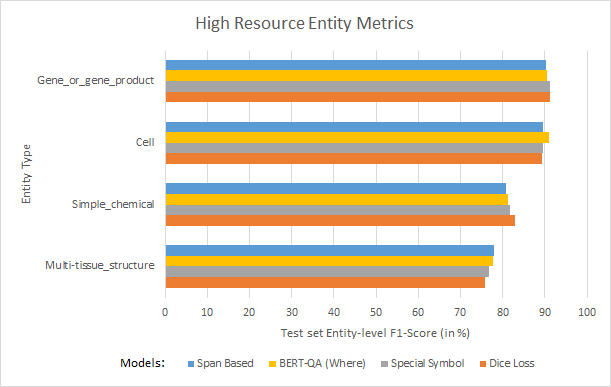
\includegraphics[scale=0.5]{../thesis/high_resource_entity_metrics}
    \caption{Test set Entity-level F1 scores for high resource entities in \texttt{BioNLP13CG} dataset}
    \label{fig:high_resource_entity_metrics}
\end{figure}

\begin{figure}
    \centering
    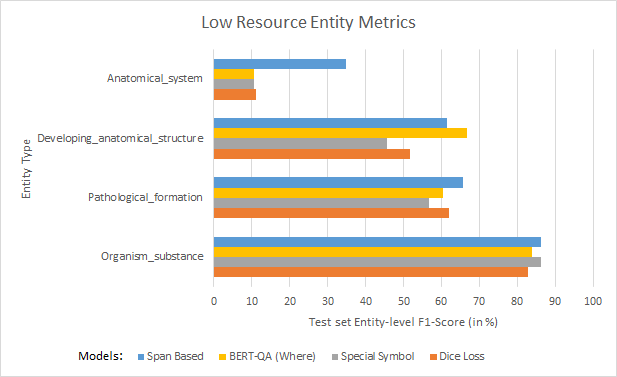
\includegraphics[scale=0.5]{../thesis/low_resource_entity_metrics}
    \caption{Test set Entity-level F1 scores for low resource entities in \texttt{BioNLP13CG} dataset}
    \label{fig:low_resource_entity_metrics}
\end{figure}

\fi
